\section{System Design}
\label{ch:system-design}

\epigraph{That men do not learn very much from the lessons of history is the most important of all the lessons that history has to teach.}{Aldous Huxley}

\subsection{System Architecture Diagram}
\begin{figure}[h]
\caption{System Architecture}
\centering
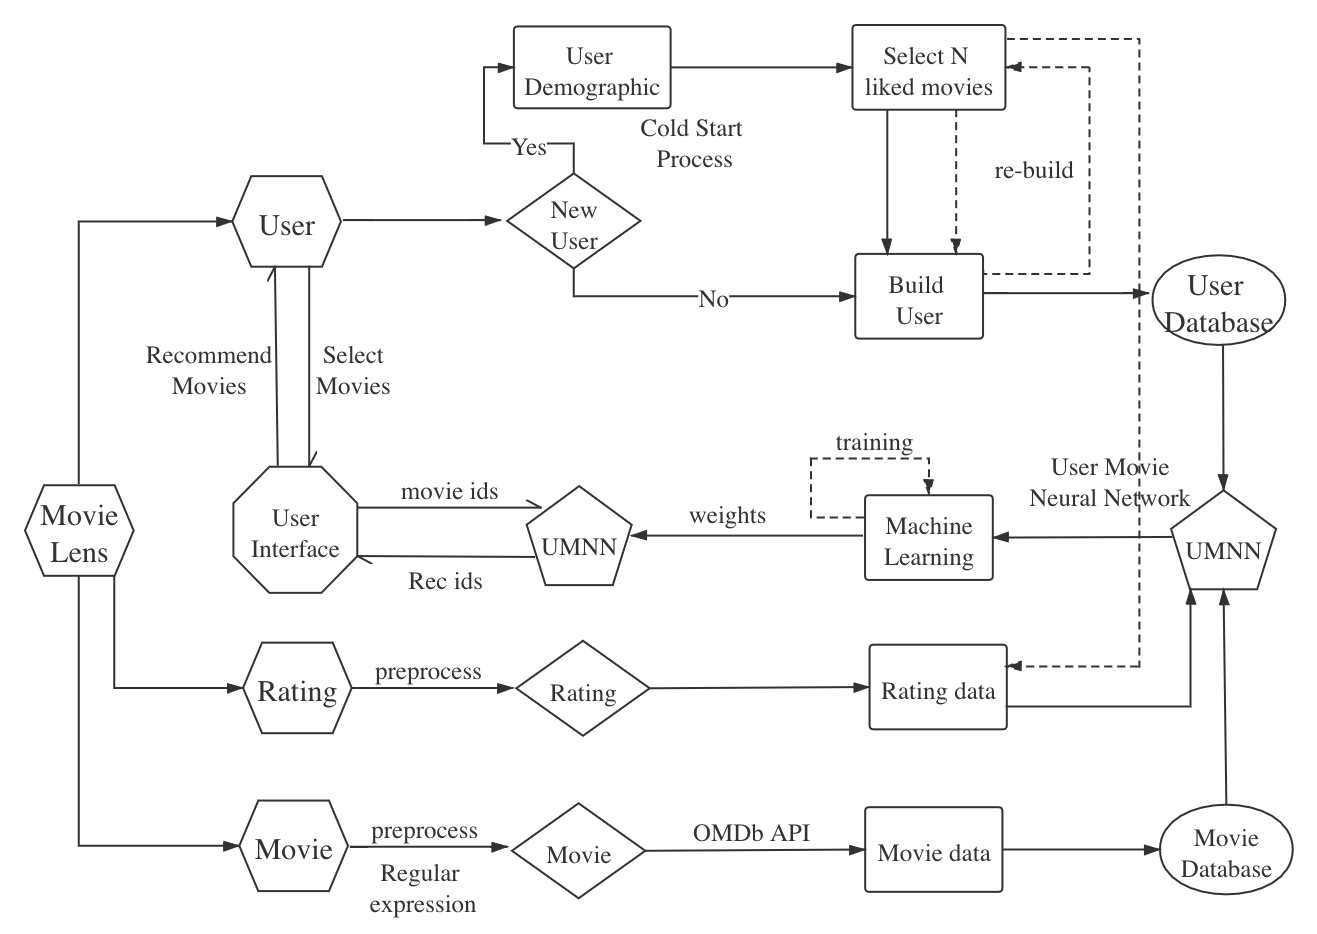
\includegraphics[width=1.0\textwidth]{system_architecture}
\end{figure}
\subsubsection{MovieLens Dataset}
%build user database and movie database
We use the MovieLens dataset from the GroupLens Research Group at the University of Minnesota. The MovieLens 1M dataset is used as the data source in this paper. It contains 1 million ratings of 4,000 movies from 6,000 users. It is divided into three tables: movie ratings, movie metadata (genre style and age), and demographic data about users (age, zip code, gender, and occupation).
\subsubsection{4 Data Tracks}
In the system architecture diagram. The two outputs from the MovieLens extract the movie table and rating table as the input of the movie module, and extract the user table as the input of the user module. The user and the movie, respectively, represent two paths, which represent the behavior trajectory when a user or a movie is entered in the system. This paper divides the entire recommendation system into four parts according to the business path, which are the user data track, movie data track, rating data track, and recommendation generation track. In the following paragraphs, we introduce each track separately.
\par In terms of user trajectory, each time a user comes in, it is necessary to determine whether the user is a new one. Once a new user is found, a cold start strategy will be initiated. The system will guide the user to enter relevant personal information (gender, age, occupation). Then take a series of top-N movies from the existing movie data and let the user choose some movies he likes. After selecting n movies (in the subsequent prototype, we set n to 10 for easy description and testing). The system will use the previously obtained personal information of the user and the selected n favorite movies as input to build a user portrait, that is, the "Build user" part in the system architecture diagram. If the user is not involved in the cold start problem, the user goes to the "Build User" process directly. This part of the user data is the existing user data obtained from the user table in MovieLens. In summary, the existing user data in MovieLens and newly entered user data constitute the entire user database of the system together.
\par There are two types of labeling for movies, which are the characteristics of the movie itself (name, genre, director, actor) and the behavior characteristics of the movie in the system.
\\
\\
\textbf{Movie characteristics:}
\par The properties of the movie itself do not need to be updated frequently. These data will hardly change or need to be updated after the first input into the system. The genre of the movie and its release year can be retrieved from MovieLens.
\begin{figure}[h]
\caption{UMNN Module}
\centering
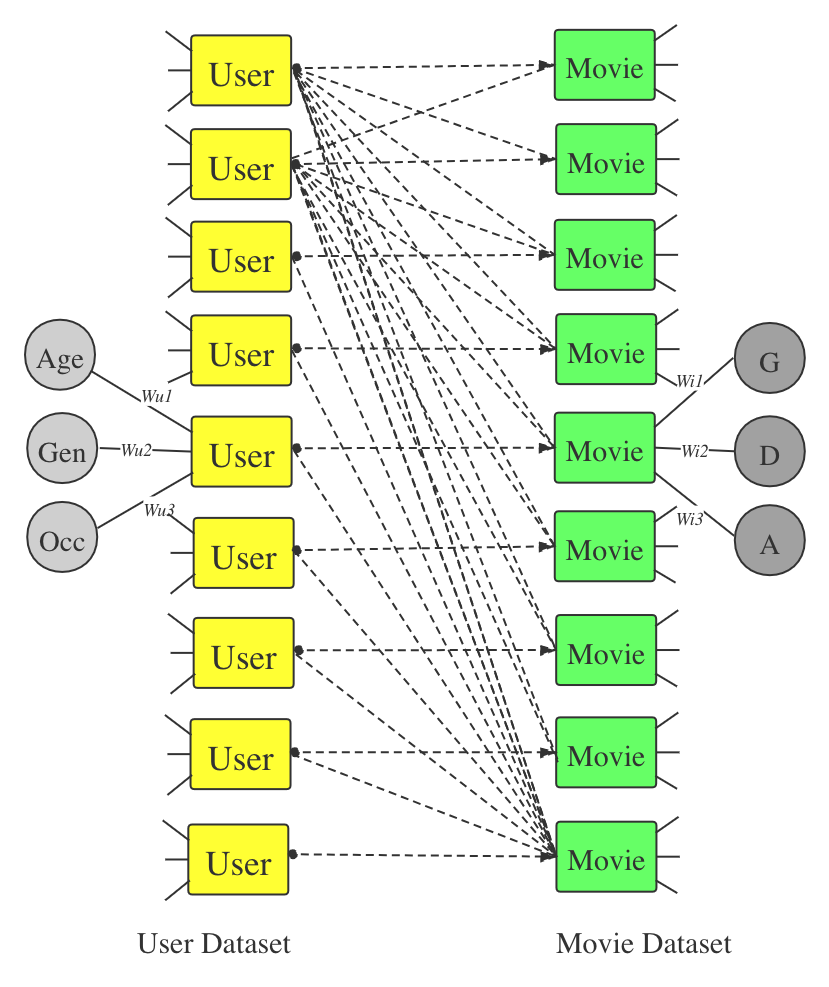
\includegraphics[width=0.5\textwidth]{UMNN_system}
\end{figure}
\par The movie data of MovieLens does not include the director, actor, writer, poster and other data of the movie. In order to obtain more useful movie metadata, so that the system we are constructing can have richer information and data to show, we use OMDb API which is a third-party RESTful web service to get movie information. The name and year of each movie are used as query inputs to obtain the director, actor, writer, and poster addresses of the movie. The new data corresponding to all movies in the entire movie table is re-integrated into a new movie table. The data items constituting the new movie table are: (iid, title, year, genre, director, actor, writer). The new movie table constitutes the "Movie Database" part in the system architecture diagram.
\\
\\
\textbf{Movie behavior characteristics:}
\par Movie behavior characteristics refer to information such as the movie being clicked and rated in the system.
\par When the movie and user characteristics are collected, the "Movie Database" and the "User Database" are formed. These two components can be combined to build a model training set. All data in user database and movie database are structured as shown in the figure UMNN Module. The data structure in the rating table contains someone user's rating of someone movie. The data of the rating table is used as a mapping from the user dataset to the movie dataset. All user nodes and movie nodes that are related in the rating table are connected. All connections in the user dataset and movie dataset have weight values, and their initial value is set to the user's rating of the movie. In summary, the training set UMNN in the system architecture diagram is finally molded. With some machine learning algorithms provided by pytorch, by multiple rounds of training on UMNN, a UMNN with a series of new weights after fitting is constructed. The UMNN model is used as the core module of the recommendation system. When the user selects N movies he likes in the User Interface, the User Interface sends the selected movie id list as input to the UMNN, and the UMNN sends the recommended id list to the User Interface, and the User Interface finally shows the recommended movies' Information.


\subsubsection{Frontend and Backend}
Flask is a web micro-framework implemented by Python. The "micro" means that Flask aims to keep the code concise and easy to extend, allowing developers to quickly implement a website or web service using the Python language. It is currently a very popular web framework that uses the Python programming language to implement related web service. Based on Werkzeug and Jinja's lightweight WSGI web application framework, the main feature of the Flask framework is that the core structure is relatively simple, but has strong extensibility and compatibility. Programmers can use Python to quickly implement a website or web service.
\par Compared with other lightweight web frameworks, the Flask framework has good extensibility, has a flexible Jinja2 template engine, and improves the reuse rate of frontend code. This is irreplaceable by other web frameworks. In fact, the frontend and Backend development can be done in Flask with Python at one time. The template and route modules provided by Flask serve as the frontend and backend functions in the traditional network architecture. We use sqlite3 lightweight database to store some data that needs to be persisted. The entire frontend and backend and database architecture is very lightweight and concise, as shown in the figure.
\begin{figure}[h]
\caption{frontend and backend}
\centering
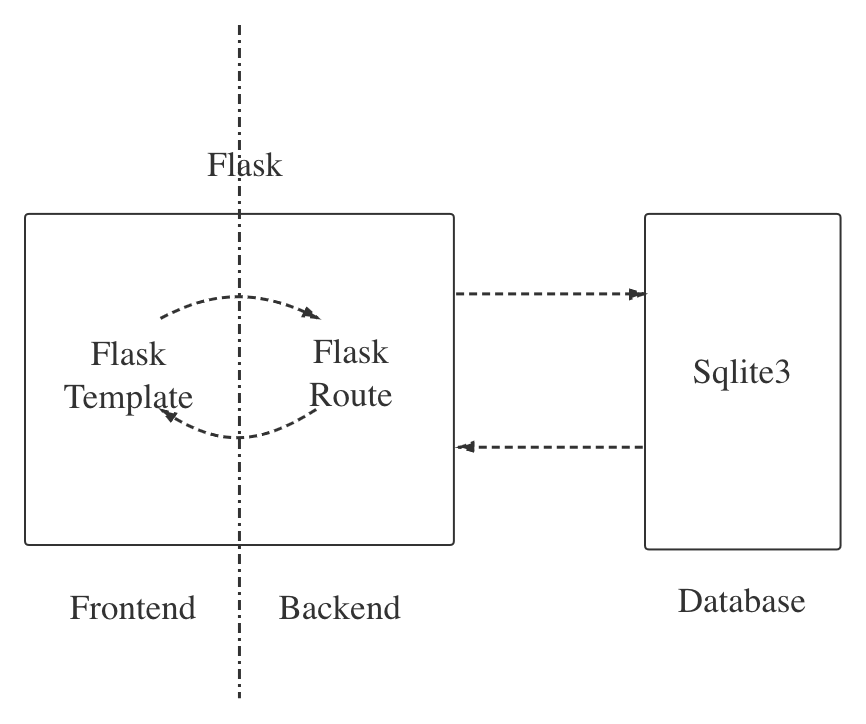
\includegraphics[width=0.8\textwidth]{frontend_backend}
\end{figure}
\par In our entire system, the development language for machine learning algorithms and data processing operations is also Python, which is one of the reasons we chose it as the web development language and the Flask framework as the web framework. The entire system is developed by a unified language, which makes the whole development and later maintenance extremely convenient and clear.
\par The basic operating mode of Flask is to assign a view function to a URL in the program. Whenever a user accesses this URL, the system will execute the view function bound to the URL in the route module, obtain the return value of the function, and display it on the browser. Usually this return value is the parsed html code. its working process is shown in the figure.
\begin{figure}[h]
\caption{Flask working process}
\centering
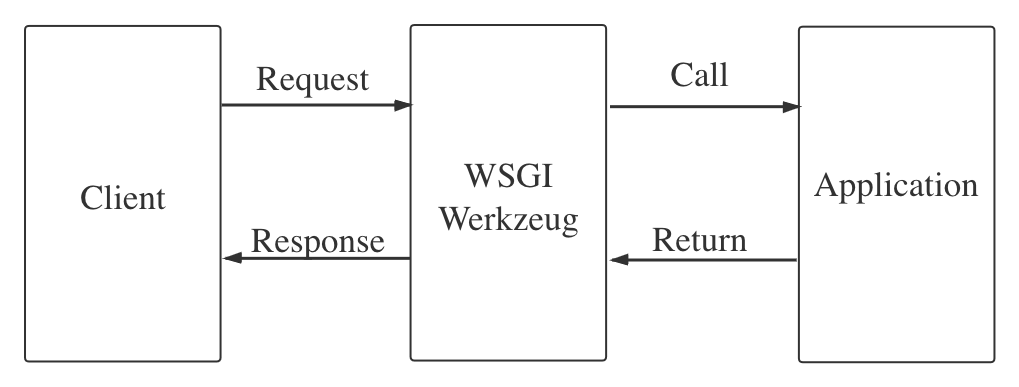
\includegraphics[width=0.8\textwidth]{flask_working_process}
\end{figure}
\par The Web Server Gateway Interface (WSGI) has been used as a standard for Python web application development. WSGI is a specification for a common interface between a web server and a web application.
\par Werkzeug is a WSGI toolkit that implements requesting service, responding objects, and building some utility functions. It makes that possible to build web frameworks on top of it. The Flask framework embeds Werkzeug as one of its foundations.
\par Jinja2 is a popular template engine for Python. The web template module combines templates with specific data sources to render dynamic web pages.

\subsubsection{User Initialization}
From a massive content library, the recommendation system recommends products that the user may like based on the user's current context information and past behavior. If a user's past behavior is empty, that is, the user's past behavior has not been recorded by the system, or he is simply a new user. A cold start problem occurs in this case.
\begin{figure}[h]
\caption{Cold start process}
\centering
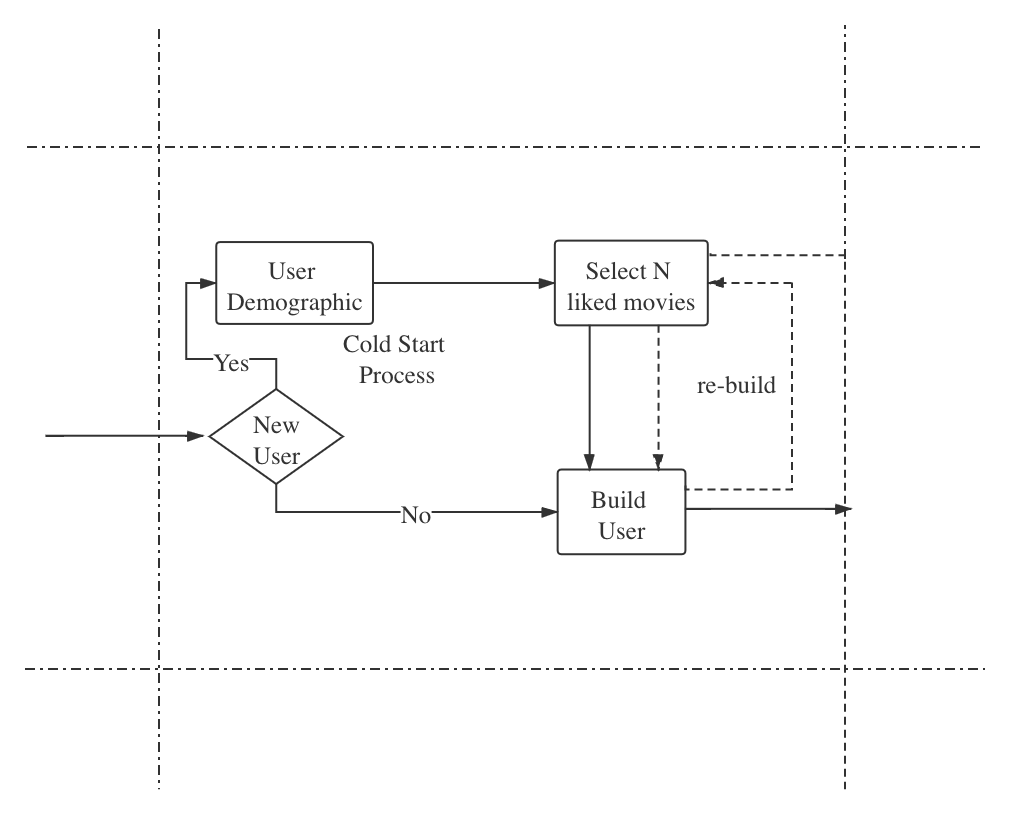
\includegraphics[width=0.6\textwidth]{cold_start_process}
\end{figure}
\par The cold start problem of the movie recommendation system can be classified into new user cold start problem and new item cold start problem.
\\
\\
\textbf{new user cold start problem: }
\par lack of personal information data for new users, lack of records of people's interaction with movies, that is, visit clicks and ratings data.
\\
\\
\textbf{new item cold start problem: }
\par After the new movie is added to the system, due to the lack of visits, the recommendation will be inaccurate, even affects the chances of new items being recommended, and then continue to affect the access to new items, resulting in negative feedback. This will lead to a popularity bias problem. Movies that were originally popular are more likely to get most recommendations, and movies that have fewer new visits are less likely to be recommended.
\par Our system data comes from MovieLens. For the part of movie data, the movie data from MovieLens can be directly inputted into the system, so this paper does not involve the new item cold start problem. About the user data part, the user data in MovieLens can be used as the source of startup data. Only when a new user uses this system, a cold start strategy is needed. The specific steps have been described in the previous section. To summarize, the new user needs to enter relevant personal information (gender, age, occupation) and choose some movies he likes from a series of top-N movies. After the selecting procedure is completed, the previously obtained personal information and the selected n favorite movies are inputted to build a user portrait.
\par The method to solve the cold start problem is usually to obtain the demographic data of the new user, guide the user to interact with the system, record the user behavior, and then map the user behavior attributes to the attribute space. So that the new user can be associated with the existing user. That is, the new user node is associated with some movie nodes in the movie dataset, and at the same time, the new user node is indirectly associated with the existing user nodes in the UMNN by these movie nodes.
\par When solving the cold start problem, there are usually two problems to be aware of.
\par The first problem is that the data generated by user behavior, in cold start process, has sparse attributes. In large-scale application systems, users need to interact with a large number of items. For a specific user, there are only few interactions in the system, and the interaction with the item may be even less. So the user-item matrix will be very sparse. To deal with the sparseness of matrices, we can construct more efficient data structures, compress sparse rows and columns, or reduce dimensions through methods such as PCA and SVD.
\par The second problem is efficiency. The recommendation system is an online system. It needs the ability of immediateness and instant feedback. The user does not want or accept long waits and too many useless interactions. We want to guide users through as few as possible but sufficient operations to obtain as much and as effective user behavior data as possible. It will not cause users to have a bad interactive experience because of tedious and redundant operations, but also can quickly and accurately construct user behavior portraits.

\subsection{Recommendation Strategy}
\subsubsection{Recommendation Style}
\begin{itemize}

\item[(a)]\textbf{Popularity-Based}\\
There are two reasons for recommending based on popularity. First, popularity often represents the important characteristics of a product. Some users utilize extensive sources of information before making decisions to choose a movie, however, the others depend on simple and limited sources of information. But they all will be affected by the popularity of movies to some extent. Second, the popularity of a movie greatly influences user's decisions. From a psychological perspective, when recommending popular movies to users, even if they are not the type the user likes, users usually subconsciously give these movies a higher rating\cite{ahn2006utilizing}. So popularity-based recommendation is a very important and simple method in the early days. In this paper, popularity-based method is used as the basis for the other four recommendation methods.
\item[(b)]\textbf{User-Based}\\
\begin{figure}[h]
\caption{user-based recommendation strategy}
\centering
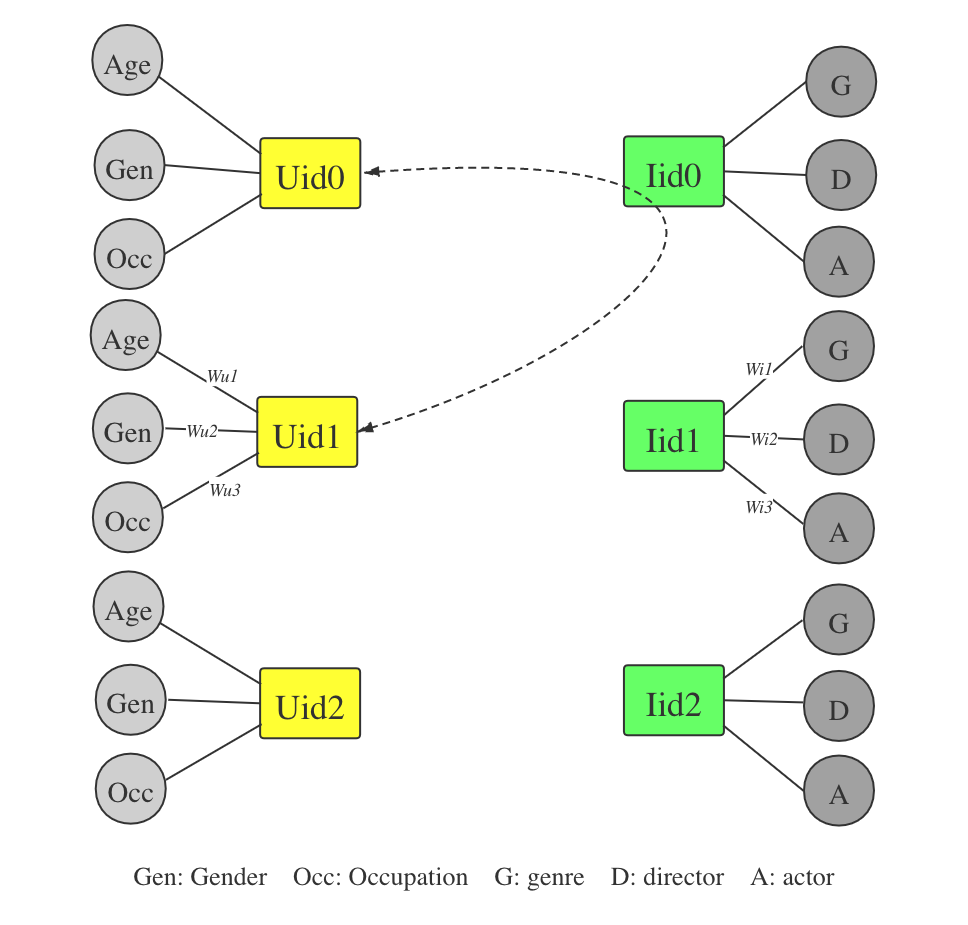
\includegraphics[width=0.5\textwidth]{neural_network_user_based}
\end{figure}
The user-based recommendation strategy more considers the interests of new user and other users with the same hobbies, recommends items that other users like / visited to the new user, and has little to do with new user's current behavior.What will be recommended to a new user, depends on what the other users have visited before. The recommended items are the favorite items of users with the same hobby, so it has a hotspot effect. it can recommend the items that the other users have just visited. It has strong real-time performance, especially the newly introduced hot spots, which can spread quickly and solve the cold start problem of new-item.
\item[(c)]\textbf{Item-Based}\\
\begin{figure}[h]
\caption{item-based recommendation strategy}
\centering
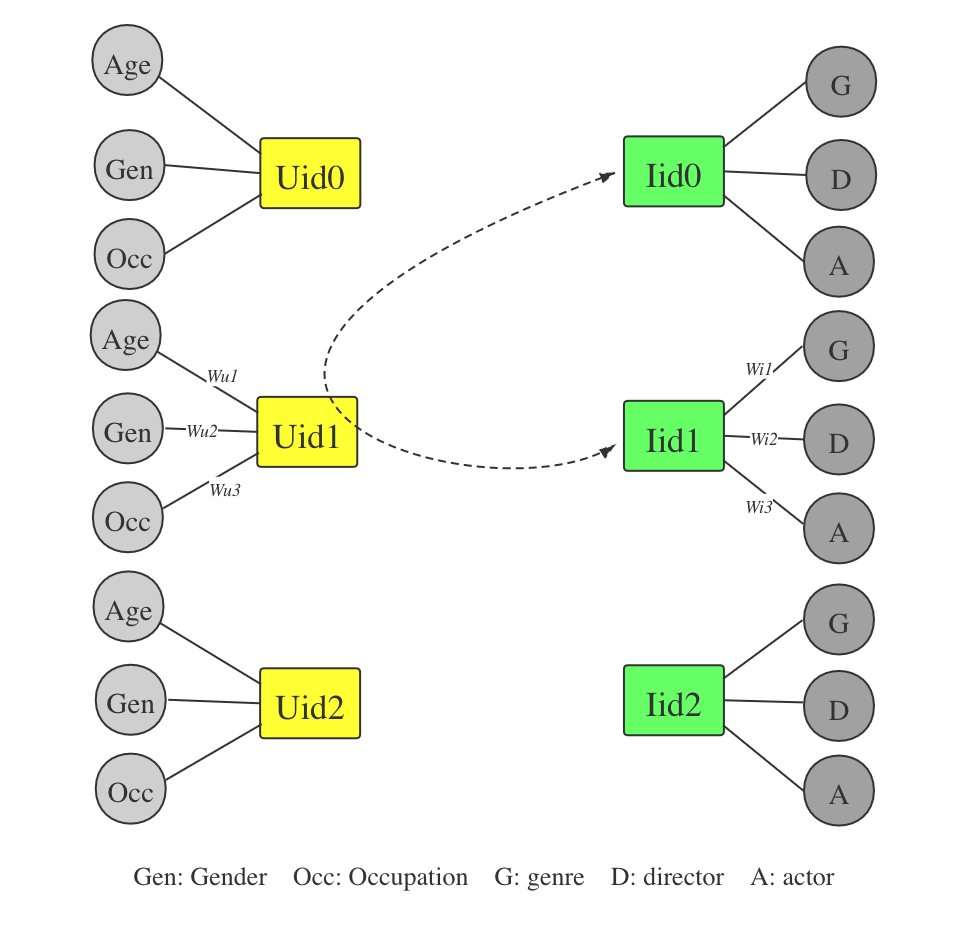
\includegraphics[width=0.5\textwidth]{neural_network_item_based}
\end{figure}
Item-based mainly uses users' historical interests to make recommendations. Recommending items that are similar to the user's history. This method has a lot to do with the user's current behavior. The similarity between the item recommended to the user and the item previously selected by the user is understandable by the user, which is called Interpretable. Most of the recommended items are not popular, but are related to the interests of users. This recommendation method has the highest accuracy when the user's interest is long-term and fixed. The significance of Item-based recommendation is to help users find items related to their interests. The recommended item is not related to user identity, so it is better to solve the problem of new users.
\par Badrul et al.\cite{sarwar2001item} compared the performance of user-based and item-based and demonstrated that the item-based algorithm provides better quality of prediction than the user-based algorithm.
\item[(d)]\textbf{Demographic-Based}\\
\begin{figure}[h]
\caption{demographic-based recommendation strategy}
\centering
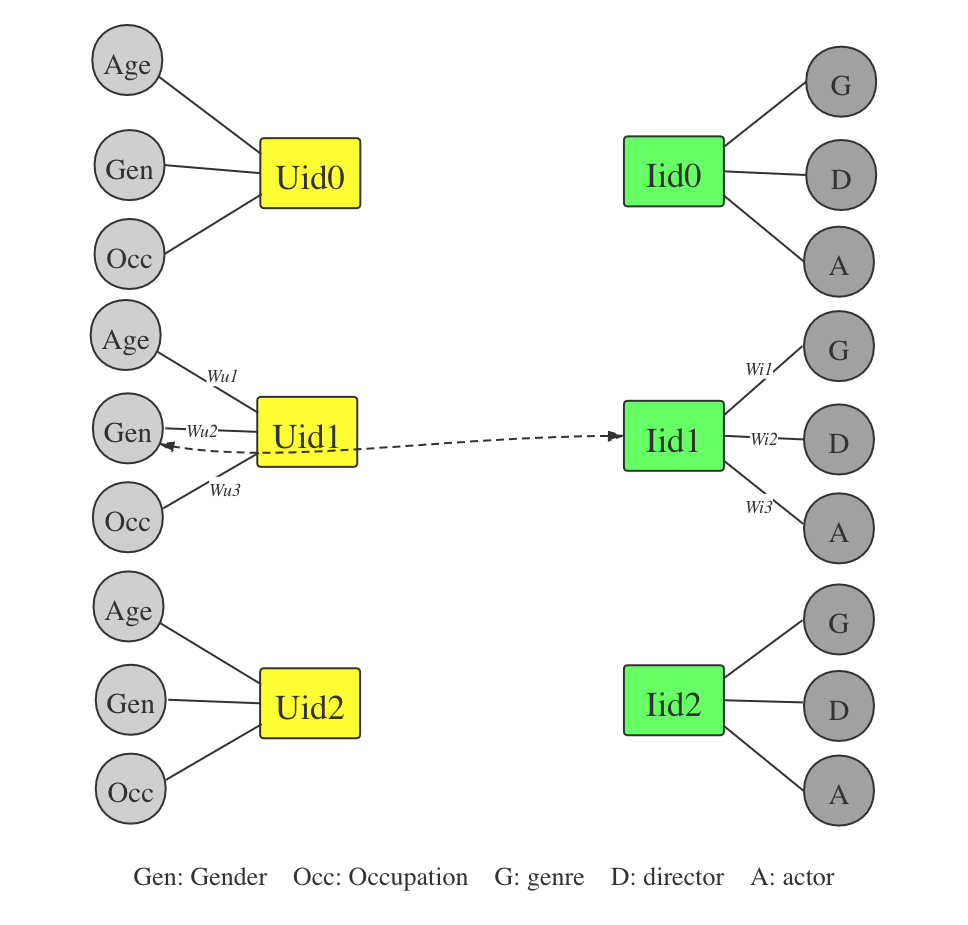
\includegraphics[width=0.5\textwidth]{neural_network_demographic_based}
\end{figure}
According to the basic information of the system user, find out the relevance of the user, and then make recommendations. At present, it is rarely used alone in large systems, and it is usually used in combination with other recommendation algorithms. The usual method is to classify the user based on the user's registration information, and then recommend to the user the items in the category to which he belongs. In this paper, we use gender, age and occupation of user as feature of demographic-based recommendation method.
\item[(e)]\textbf{Content-Based}\\
\begin{figure}[h]
\caption{content-based recommendation strategy}
\centering
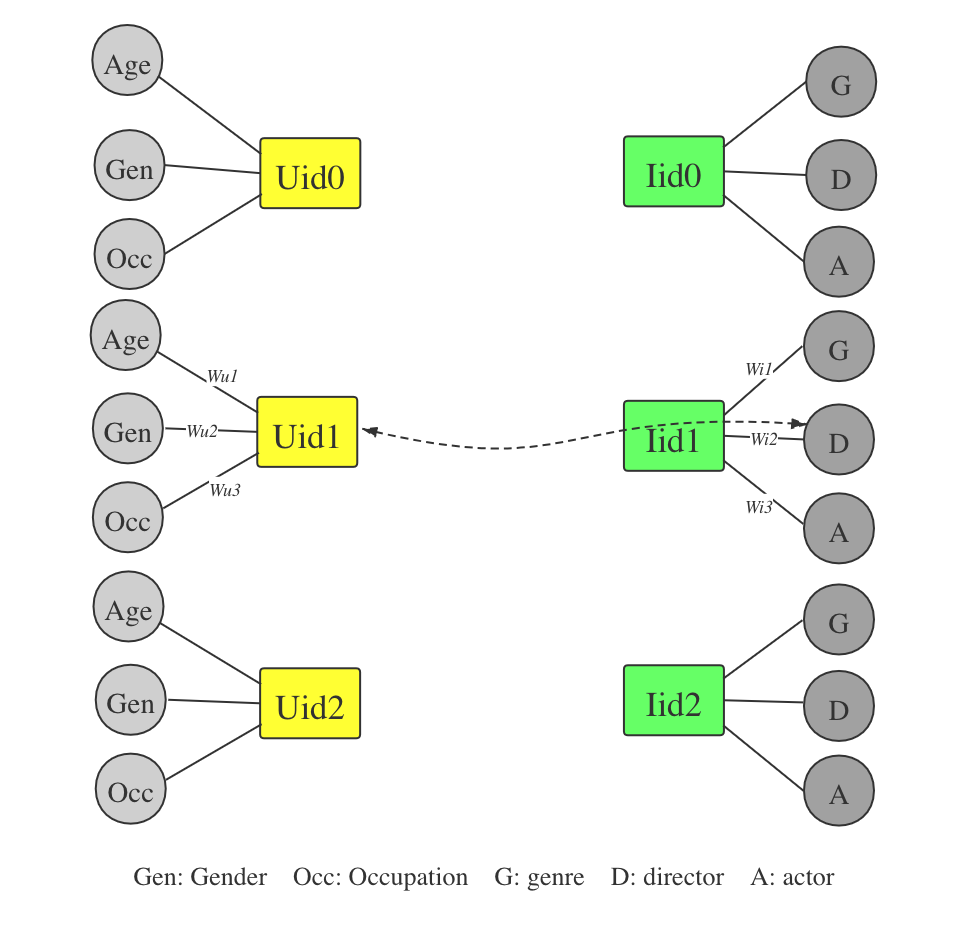
\includegraphics[width=0.5\textwidth]{neural_network_content_based}
\end{figure}
Based on the user's past browsing history, make recommendations to the user that he/she has not viewed. Recommendations are generally based on keywords or content features. For example, if a user has previously chosen to be interested in a certain director's movie, the user will be recommended with the other movie works of this director. The advantage of this method is that there is no popularity bias, items with rare features can be recommended, and user content characteristics can be used to provide recommendation explanations. The disadvantage is that the content must be machine-readable and meaningful, and the features of the recommended content need to be archived in advance.
\par Recommend movies that are similar to movies that users have liked. It is mainly based on the comparison of movie attribute information and user portrait information. The core problem is how to establish the association between movie attributes and user information. it assumes that users will rate items having alike features similarly\cite{safoury2013exploiting}.

\end{itemize}

\par For various reasons, it is easier to collect the user's past behavior than to collect user information, but CF-based (user-based and item-based) has it's limitations. When the scoring is very sparse, the prediction accuracy will be greatly reduced. And the cold start of new products is also a problem for CF. In general, therefore, most of today's recommendation systems use a hybrid recommendation method.
\subsubsection{Recommendation Explanation Strategy}
In the construction of UMNN, all connection methods are recorded while the user node and the movie node are connected. When the User Interface sends a movie id list and UMNN sends a recommended id list, the corresponding connection method is transmitted to the User Interface as part of the response data.
\par We introduced the method for establishing a connection between the user node and the movie node in the Recommendation Style section. Each recommendation style can be relevant to a Recommendation Explanation Template.
\\
\begin{table}[h!]
\centering

\textbf{UserNode--MovieNode--UserNode}\\
\textbf{MovieNode--UserNode--MovieNode}\\
\textbf{DemographicFeature--UserNode--MovieNode}\\
\textbf{UserNode--MovieNode--ContentFeature}\\

\caption{Four connection methods}
\label{table:1}
\end{table}
The four recommended methods corresponding to the four connection methods in \ref{table:1} are user-based, item-based, demographic-based, and content-based. Establish the explanation templates for these four recommendation styles in table \ref{table:2}.

\begin{table}[h!]
\renewcommand\arraystretch{1.5}
\centering
\begin{tabular}{p{80pt}p{120pt}p{100pt}p{120pt}}\toprule
 \hline
 Recommendation Style & Explanation Template & Data Template & Example \\ [0.5ex] 
 \hline\hline
 user-based & (uid\_1) is recommended with (iid\_1) because (uid\_2) is similar with (uid\_1) and (uid\_2) likes (iid\_1). & Uid\{uid-1\}-Iid\{iid1\}-Uid\{uid2\} & You are recommended with "Resurrection Man (1998)" because user 5183 is similar with you and user 5183 likes this movie.\\ 
 item-based & (iid\_1) is recommended to (uid\_1) because (iid\_1) that is similar with (iid\_2) which (uid\_1) liked before. & Iid\{iid1\}-Uid\{uid-1\}-Iid\{iid2\} & "Woo (1998)" is recommended to you because that is similar with "Ice Storm (1997)" which you liked before. \\
 demographic-based & (iid\_1) is recommended to (uid\_1) because (uid\_1)'s (DemographicFeatureType) is (DemographicFeatureValue). & Iid\{iid1\}-Uid\{uid-1\}-DFType\{type\}-DFValue\{value\} & "12 Monkeys (1995)" is recommended to you because your occupation is academic/educator. \\
 content-based & content-based: (uid\_1) is recommend with (iid\_1) because (iid\_1)'s (ContentFeatureType) is (ContentFeatureValue) & Uid\{uid-1\}-Iid\{iid\}-CFType\{type\}-CFValue\{value\} & You are recommended with "Resurrection Man (1998)" because the genre of the movie is Crime.\\ [1ex] 
 \hline
\end{tabular}
\caption{Explanation Template}
\label{table:2}
\end{table}
\subsubsection{Recommendation Explanation Adaptation Strategy}
%rule based
The quality of a recommendation system usually requires an evaluation of the entire recommendation behavior, which runs through the user's whole interaction process. A recommendation system is good or not good, which is difficult to define. The algorithm is the core of the recommendation system, while a variety of other technologies and factors have a significant impact on personalized recommendations. The excellent recommendation system is a hybrid product of algorithms, various technics, and interaction designs.
\par From the use of search engines when there is less information at the beginning of the Internet, to the use of recommendation systems after more information appears on the Internet, to the applied of interpretable recommendation systems that provide a better interactive experience, the way users obtain information is constantly improved and optimized. In this paper, we use the adaptation method, which was rarely studied in previous related papers, to further increase the interaction between the recommended content and the user, so that the user is more actively involved in the operation of the recommendation system, instead of as a simple message receiver. By allowing users to use our recommendation system multiple times, we collect the input of user behavior characteristics for each round as positive feedback to promote various aspects of the performance of the recommendation system.
\par We find some available and reasonable recommendation explanation adaptation strategies: adaptation for the way of showing, adaptation by trying to insert minority items, adaptation based on several rounds of user feedback.
\\
\textbf{Adaptation for the way of showing:}\\
Adapt the shown of the explanation. The original movie recommendation explanation of the system is an understandable sentence using natural language, but sometimes the user is not interested in the uniform text description, and it is not necessary for the user to receive all the text information in the recommendation explanation. From linguistics, we know that the user only needs to read a few keywords, In most cases, he can connect, arrange, extend and imagine the keywords to understand the meaning of recommendation explanation.
\par We propose a possible solution for the adaptation view: use word cloud. We can combine the movie?s explanation content with the movie ?s metadata on wikipedia and OMDb. After doing some data processing, a word cloud can be generated. This word cloud could contain many important movie related tags or features. user can understand the reason for recommendation by the word cloud.
\par As shown in figure, there are two word clouds for the movie "Avengers Endgame" and the movie "The Dark Knight". we can respectively get the keywords from two word clouds and know the explanation of recommendation.

\begin{figure}[h]
\caption{Word cloud}
\centering
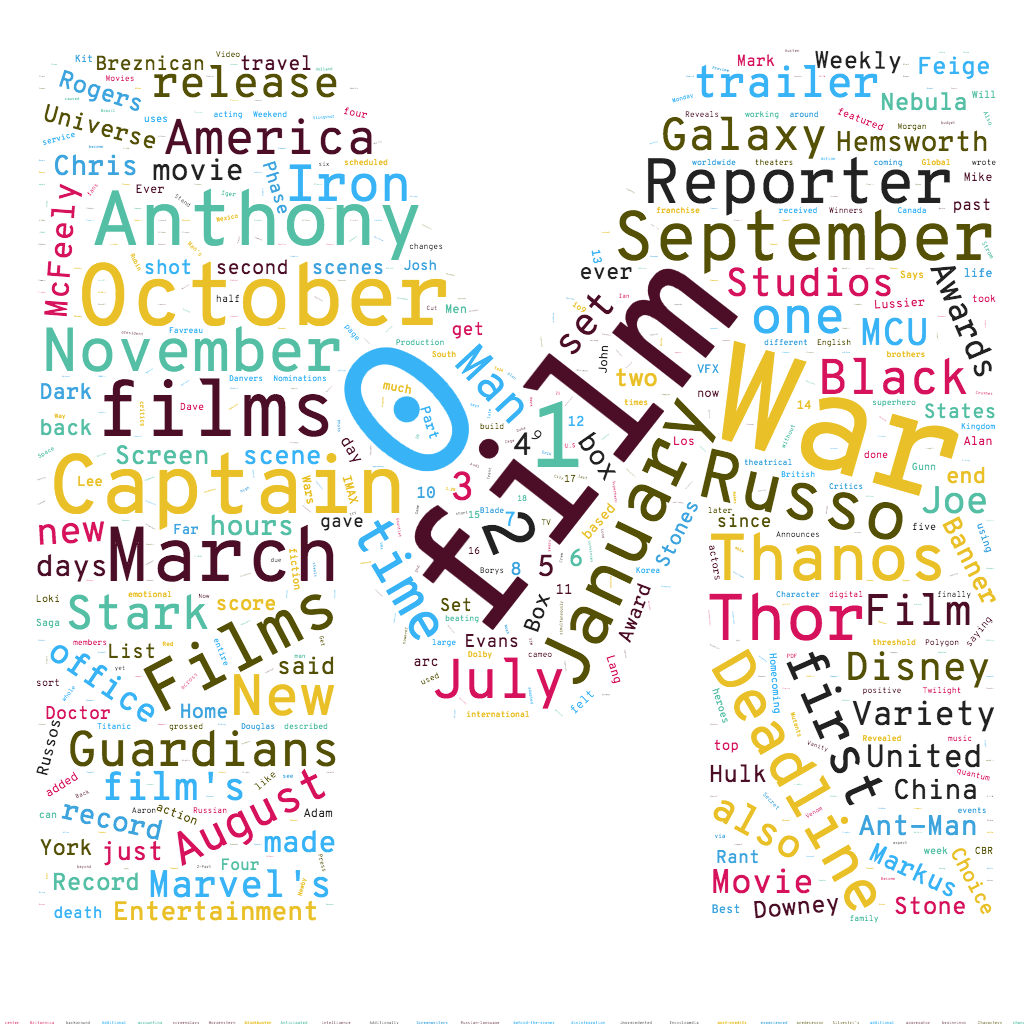
\includegraphics[width=0.4\textwidth]{avengers_endgame_flim}
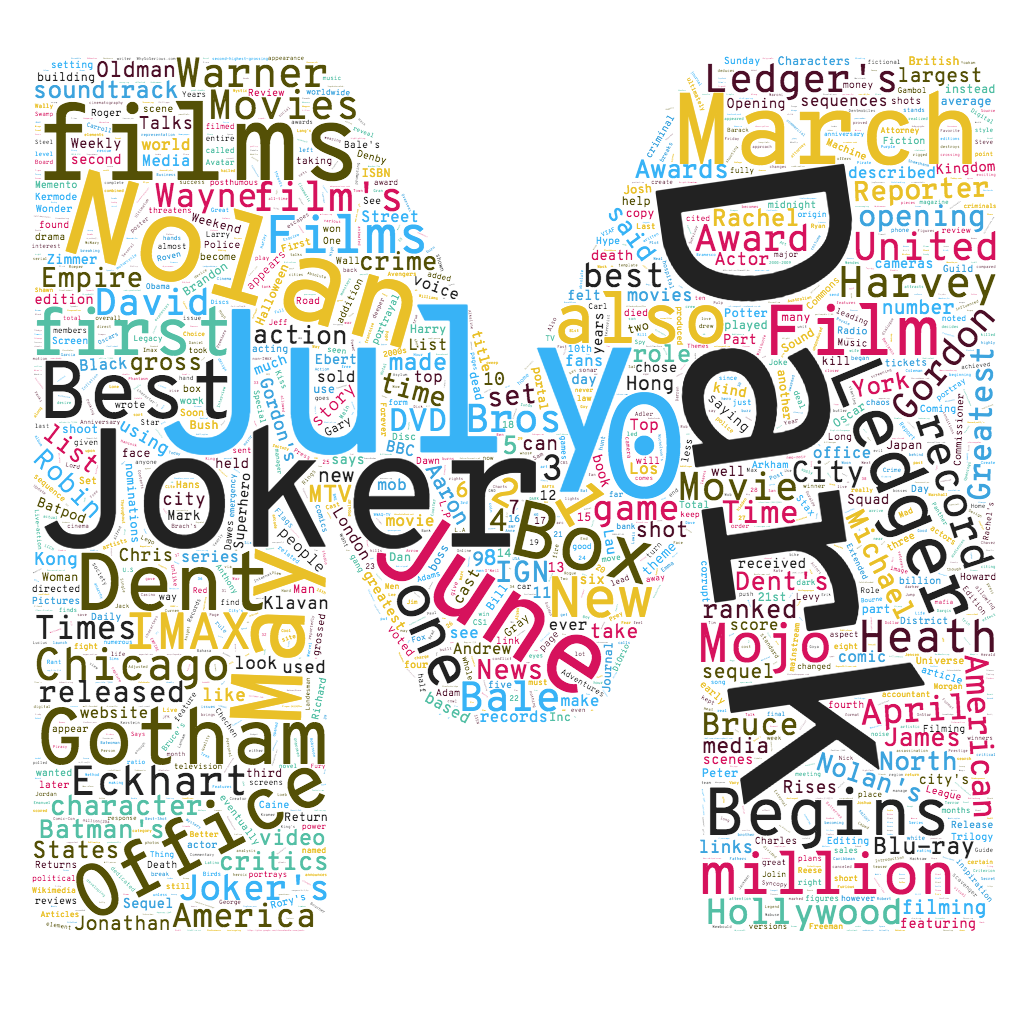
\includegraphics[width=0.4\textwidth]{the_dark_knight_film}
\end{figure}
\textbf{Adaptation based on several rounds of user feedback:} \\
\par The core idea of this method is to record the relevant data of each round when the user interacts with the recommendation system for multiple rounds. The previous round of interaction data is used as input data to train and modify the user's portrait of the user stored in the system.
\par Taking the ratio of different recommended styles as an example, we can establish an adaptation rule:

\begin{algorithm}[H]
\SetAlgoLined
\KwResult{propotion }
  \[ \bar{score}(Sum) = \frac{\sum_{i=0}^{n}rating_{i}}{n} \] \
  \[ \bar{score}(IUI) = \frac{\sum_{i\in IUI}rating_{i}}{|IUI|} \] \
  \[ \bar{score}(UIU) = \frac{\sum_{i\in UIU}rating_{i}}{|UIU|} \] \
  \[ \bar{score}(IUDD) = \frac{\sum_{i\in IUDD}rating_{i}}{|IUDD|} \] \
  \[ \bar{score}(UICC) = \frac{\sum_{i\in UICC}rating_{i}}{|UICC|} \] \
 \While{\[ count_{sum}==10 \]}{
  \[ count_{IUI}  \mathrel{+}= func_{propotion}(\bar{score}(IUI)-\bar{score}(sum)) \] \
  \[ count_{UIU}  \mathrel{+}= func_{propotion}(\bar{score}(UIU)-\bar{score}(sum)) \] \
  \[ count_{IUDD}  \mathrel{+}= func_{propotion}(\bar{score}(IUDD)-\bar{score}(sum)) \] \
  \[ count_{UICC}  \mathrel{+}= func_{propotion}(\bar{score}(UICC)-\bar{score}(sum)) \] \
  \If{\[ count_{x} < 0 \]}{
    \[ count_{x} = 0 \] \
   }
 }
 \caption{Adaptation Rule Algorithm}
\end{algorithm}

\subsection{Machine Learning Algorithm}

\subsubsection{Tool and Library}
%weights
PyTorch\cite{ketkar2017introduction} and TensorFlow\cite{abadi2016tensorflow} are currently the most popular methods for investigating deep learning and neural networks. PyTorch is more useful for researchers, enthusiasts and Individual developers to quickly build prototype in small-scale projects. TensorFlow is more suitable for large-scale deployments, especially when cross-platform and embedded deployments are required. In our research, PyTorch was selected for its vast repository of libraries to handle dataset preprocessing, statistical analysis, plotting, and more.\cite{paszke2019pytorch}.

%\subsubsection{Neural Network Model}
%node and item
\subsubsection{Algorithm}

\begin{algorithm}[H]
\SetAlgoLined
\KwResult{ \[ P_{v_{1}} \] \[ \hat{r} \] }

\[
P_{v_{1}} = \begin{bmatrix}
 genre & actor  & ... & ... & ... \\ 
 ... & ...  & ... & ... & ... \\ 
 I_{1}& I_{2} & I_{x} & ... & ... \\ 
 V_{1} & V_{1}  & V_{1}  & V_{1} & ...
\end{bmatrix}
\ \ \ \ L_{P}\times N_{P}
\]
\\
\[
L_{P} : Length \ of \ Path
\]
\[
N_{P} : Count \ of \ Path
\]
\[
\left\{\begin{matrix}
\\ p_{1} = f_{path-encoder} (V_{genres},V_{I_{1}},V_{1})
\\ ...
\\ ...
\\ p_{N_{P}} = f_{path-encoder} (V_{director},V_{I_{N}},V_{1})

\end{matrix}\right.
\]
\[
att_{p_{1}} = \frac{e^{P_{1} \cdot A^{T}}}{e^{\sigma(p_{1}\cdot A^{T})}  +  e^{\sigma(p_{2}\cdot A^{T})}  + \cdot \cdot \cdot +e^{\sigma(p_{N_{P}}\cdot A^{T})}}
\]
\[
\textbf{h}v_{1} =  \sum_{i=1}^{N_{P}} att_{i}\cdot P_{i}
\]
\[
\hat{r} = \textbf{h}_{user}\cdot \textbf{h}_{att}^{T}
\]
 
\caption{Path Generated Algorithm}
\label{algorithm:3}
\end{algorithm}

\textbf{ \ \ }\\
\textbf{ \ \ }\\
\textbf{ \ \ }\\
\textbf{Training Weights:}\\
$ A^{T} $ in algorithm \ref{algorithm:3} is a matrix that can be trained with large amounts of data. \\
$ \sigma $ is sigmoid function.\\
The $ att_{p_{1}} $ is also called a softmax(P,a) \cite{wu2016deep}.

\subsection{User Interface Prototype} 

\textbf{UI flow:}\\
In general, the UI flow is basically the same as the user data track in the system architecture diagram. Therefore, we can analyze the input and output data flow and its logical flow required by the prototype system according to the user data track, and design corresponding modules based on the functions required by the system.\\
\textbf{Prototype:}\\
The user interface prototype is designed as shown in figure \ref{figure:12}.

\begin{figure}[h]
\caption{User interface prototype}
\label{figure:12}
\centering
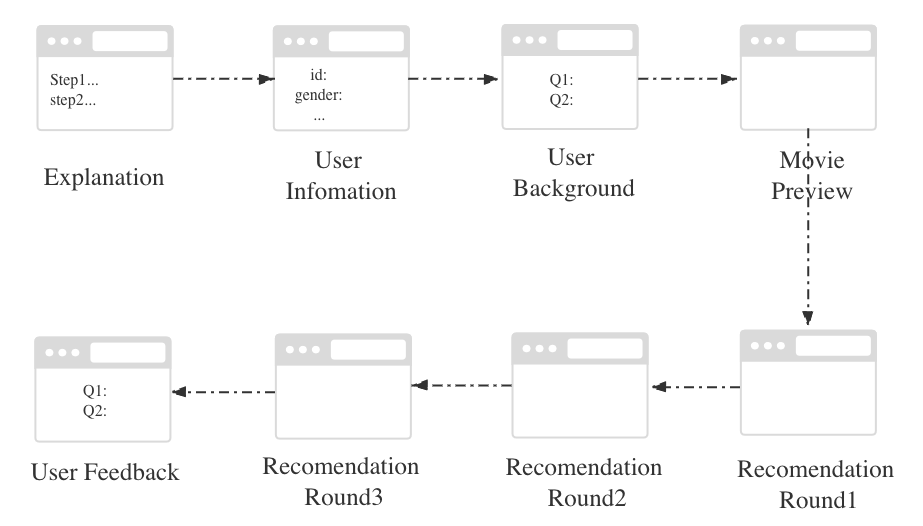
\includegraphics[width=0.8\textwidth]{prototype}
\end{figure}
\leavevmode\\


\begin{table}[h!]
\renewcommand\arraystretch{1.5}
\centering
\begin{tabular}{p{100pt}p{300pt}}\toprule
 \hline
 Page & Description \\ [0.5ex] 
 \hline
  Explanation page & Some explanations about the User Study \\
User information page &  For inputing personal data, like user id, gender, age and occupation.\\
User background page  &  The user will be asked about some background questions, like, how many does he know about Explainable Recommendation System?\\
Movie preview page  &  For building User Portraits, system will give user a series of movie posters and names. user can click to select the movies he likes from 6 options (selecting multiple, selecting none in 6 options and selecting all 6 options are allowed). Click the 'REFRESH' button to load the new 6 options. Repeat this selection process until the user has selected a total of 10 movies. \\
Recommendation round 1  &  The system will give user a series of recommendation movies and the explanations why these are recommended to the user. The user can click to select the movies he likes and give a score for the explanations. \\
Recommendation round 2  &  Same with Recommendation Round One, but the new recommendation movies are based on the user's choices and scores in Recommendation Round One. \\
Recommendation round 3  &  Same with Recommendation Round One and Two, but the new recommendation movies are based on the user's choices and scores in Recommendation Round Two. \\
User feedback page   &  The user's opinion about recommendation in the 3 test rounds.\\
  [1ex] 
 \hline
\end{tabular}
\caption{Prototype Description}
\label{table:1}
\end{table}


\cleardoublepage